\documentclass[9pt,technote]{IEEEtran} % Transactions on Robotics style
%\documentclass[12pt]{article}

%\usepackage[tight,footnotesize]{subfigure}
\usepackage{answers}
\usepackage{setspace}
\usepackage{graphicx}
%\usepackage{enumitem}
\usepackage{multicol}
\usepackage{color}
\usepackage[table]{xcolor}
\usepackage{mathrsfs}
\usepackage[margin=1in]{geometry}
\usepackage{amsmath,amsthm,amssymb}
%\usepackage{tikzpicture}
\usepackage{tikz}
\usepackage{hyperref}
%\usepackage{subfigure}
\usepackage{caption,subcaption}
\usepackage{rotating}

\begin{document}

% --------------------------------------------------------------
%                         Start here
% --------------------------------------------------------------

\title{SAM Driver \& Software Architecture overview}%replace with the appropriate homework number
\author{Dr. Nils Bore\\ %replace with your name
Robotics, Perception and Learning Lab, KTH, Stockholm\\
nbore@kth.se} %if necessary, replace with your course title

\maketitle
%Below is an example of the problem environment

\begin{abstract}
This is a design document intended to guide the development
of the software architecture for the SMARC SAM AUV.
We detail the interface of the hardware components to the
software stack, and propose an interface between
the basic software components. The design document
is accompanied by implementations of several of the
proposed components, as found in the repository
\texttt{gitr.sys.kth.se/smarc-project/sam\_drivers}.
\end{abstract}

%\section{Hardware Overview}

\section{Architecture Overview}
\label{overview}

The SAM AUV platform is designed to use two identical ARM processors as its main computers.
These will be referred to as the \textit{base} and \textit{science} computers respectively.
In this document we are mainly concerned with the software architecture on the \textit{base}
computer, and any discussion refers to that unless otherwise mentioned.
The base computer communicate with sensors and actuators (henceforth referred to as \textit{devices})
via the CAN bus protocol. Attached to most devices are \textit{Teensy} microcontrollers, which
handle the interfacing with the CAN bus network. The microcontrollers are also responsible for
synching the time of all devices to that of the computers.

\section{ROS Middleware}
\label{ros}

\textit{The Robot Operating System} (ROS)\footnote{\texttt{https://ros.org/}} is a so called \textit{middleware}, that allows different processes on
a computer or network to communicate with each other in different ways.
It also provides ways of organizing and running software. ROS allows the transmission of data types,
called ROS \textit{messages}, between components via a publisher/subscriber model.
A large collection of message types are already
provided through the ROS software distribution, but you may also define new message types.
The advantage of using provided or standardized message types is that the ROS community
already provides tools for operating on many of these types,
and that you can display them in the \textit{Rviz} visualization tool.

\section{UAVCAN Protocol}
\label{uavcan}

UAVCAN\footnote{\texttt{https://uavcan.org/}} is a high-level protocol defined on top of CAN bus. It allows for easy and robust
communication of data types over a CAN bus network. Similar to ROS, UAVCAN defines its
own message types, and allow the user to extend the already exiting types with new messages.
UAVCAN \textit{nodes} are responsible for transmitting and receiving messages over the network.
They may run both on full-fledged processors such as that of the base computer, or on microcontrollers.
UAVCAN also provides tools for synching the time of the attached nodes.

\section{Components}
\label{components}

\subsection{Devices \& Teensys}

As stated the Section \ref{overview}, most sensor and actuators are hooked up to a Teensy microcontroller.
The microcontrollers all provide a UAVCAN node that may provide both subscribe and publish
functionality, depending on the capabilities of the attached device.
Note that ROS and UAVCAN messages, while similar, can not be defined in a way
as to be shared between the two. To get data from the Teensys into the ROS middleware
on the base computer, we therefore need to define an interoperability layer.

\subsection{uavcan\_ros\_bridge}
\label{bridge}

\begin{sidewaysfigure*}
% Graphic for TeX using PGF
% Title: /home/nbore/Workspace/sam_ws/src/sam_drivers/sam_architecture/img/sam_architecture.dia
% Creator: Dia v0.97.3
% CreationDate: Thu Sep  6 16:46:12 2018
% For: nbore
% \usepackage{tikz}
% The following commands are not supported in PSTricks at present
% We define them conditionally, so when they are implemented,
% this pgf file will use them.
\ifx\du\undefined
  \newlength{\du}
\fi
\setlength{\du}{15\unitlength}
\scalebox{.6}{
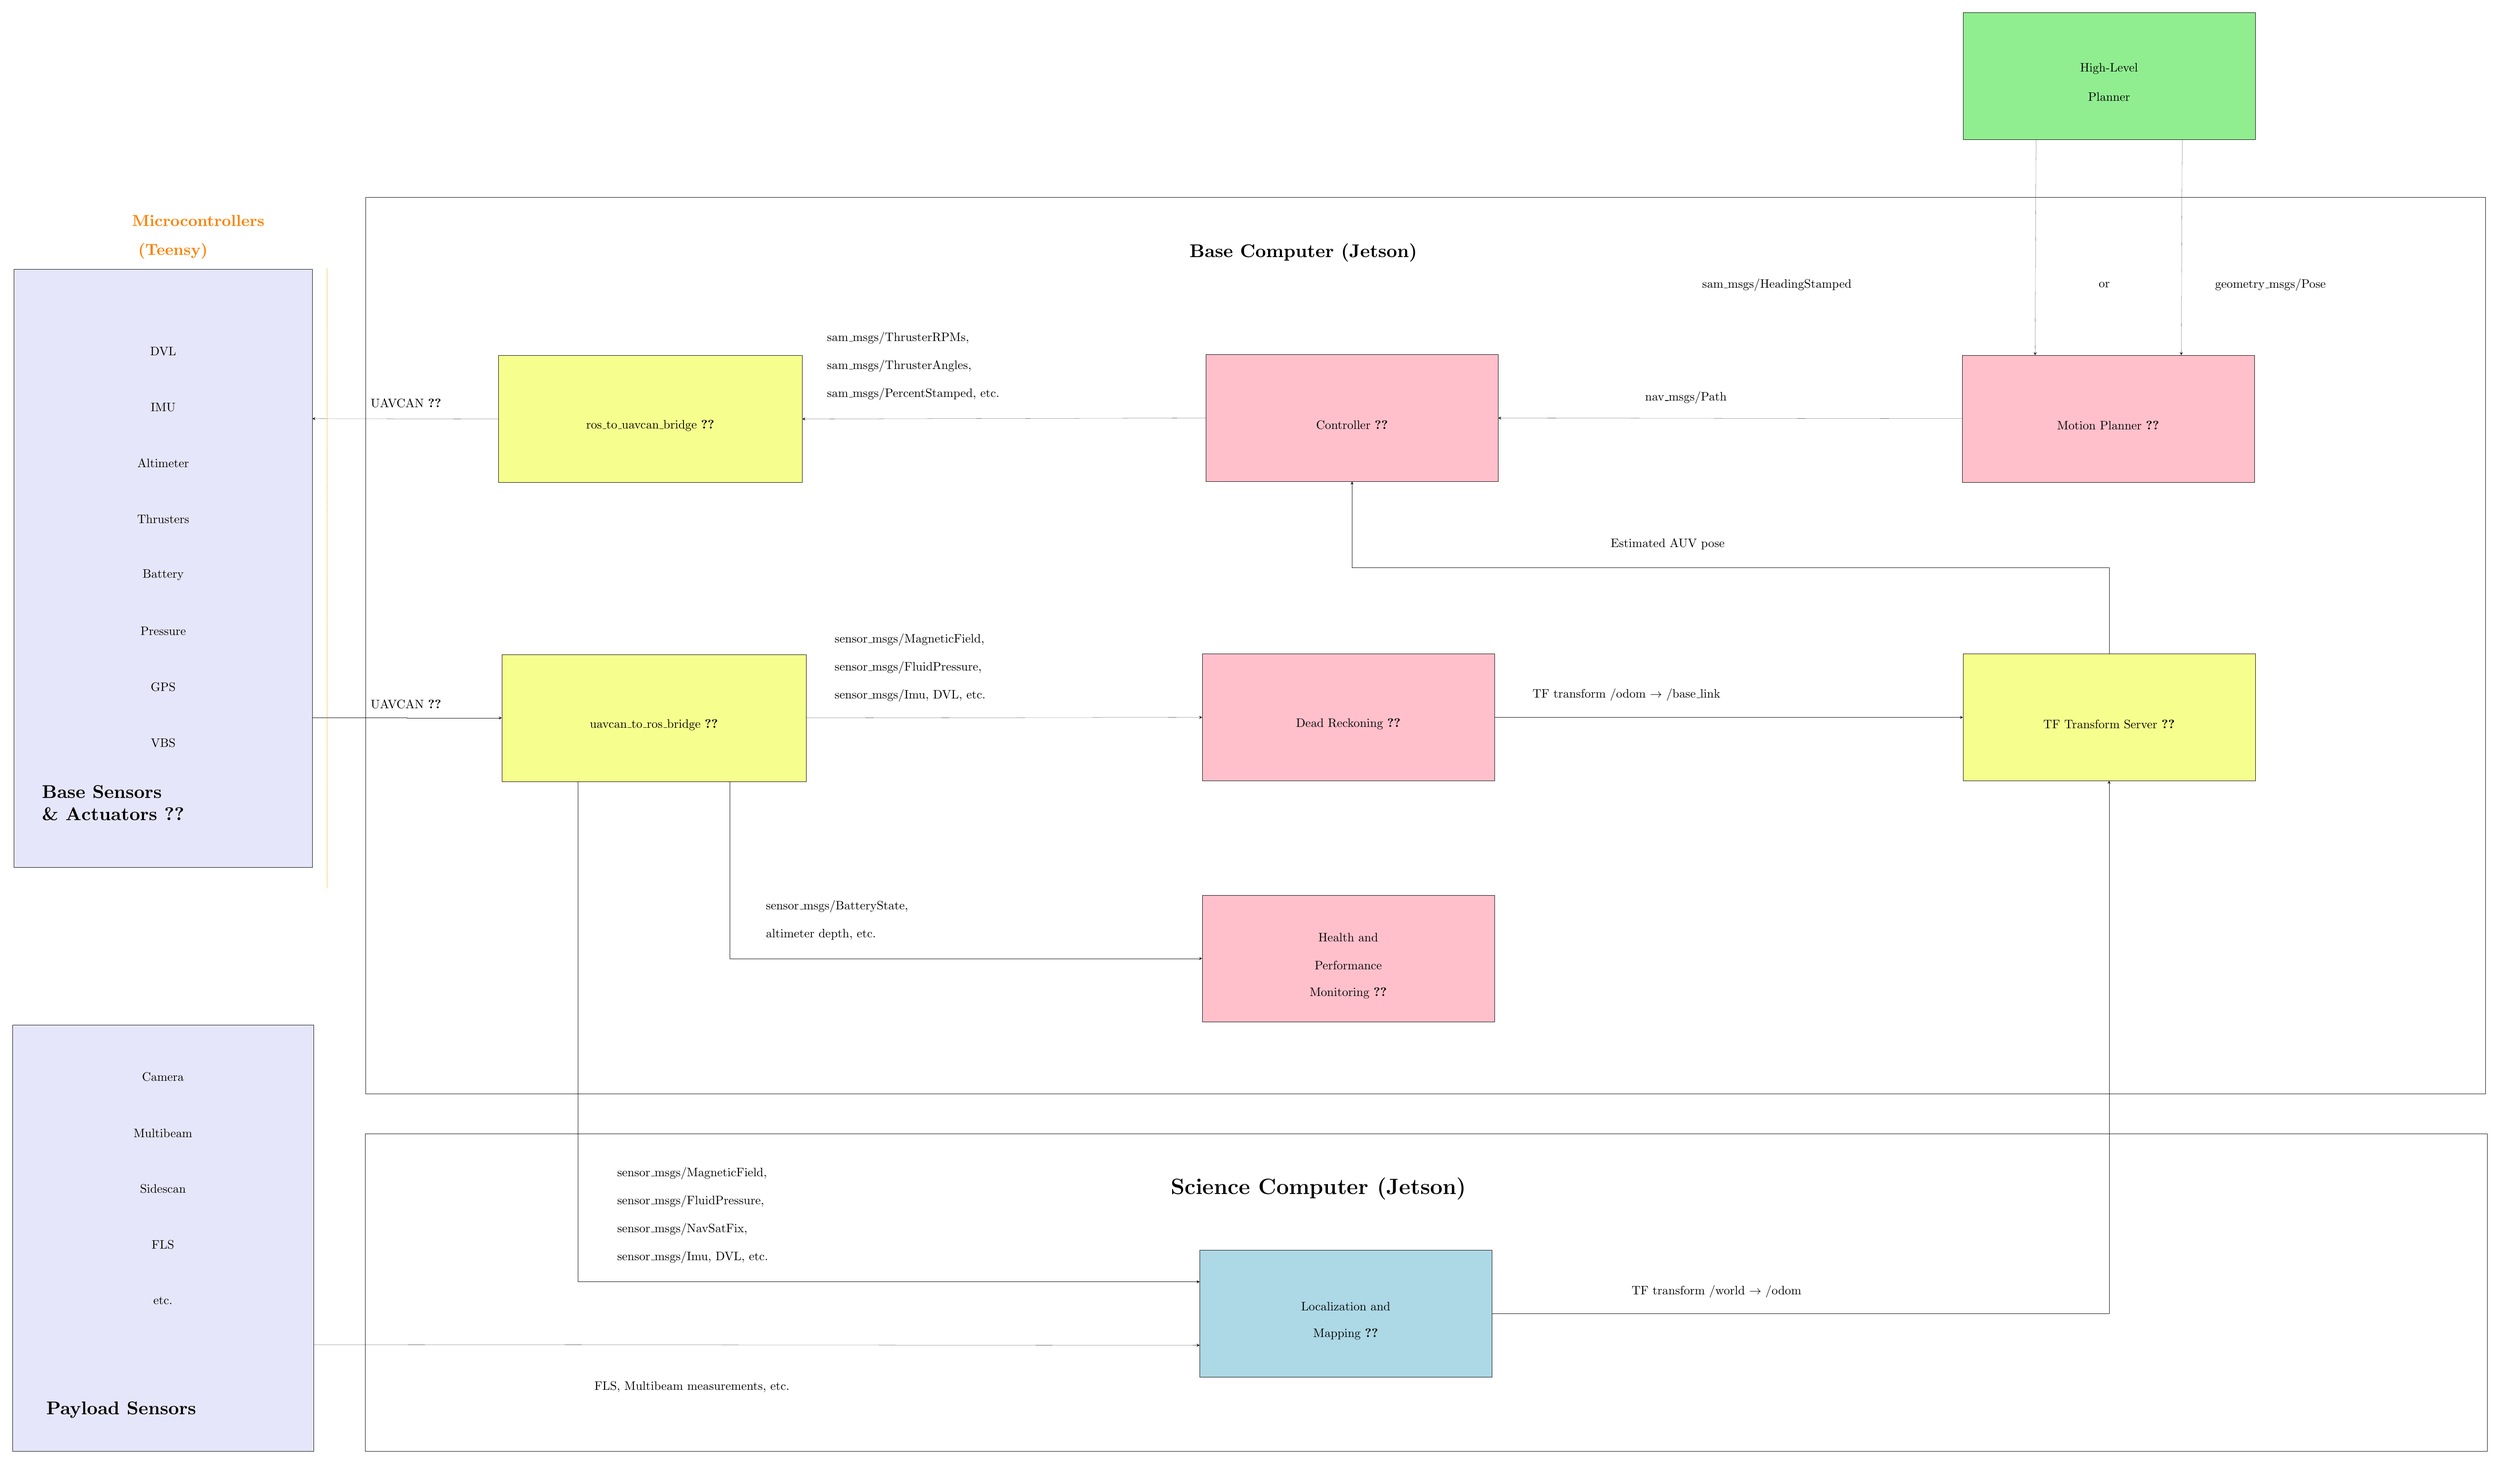
\begin{tikzpicture}
\pgftransformxscale{1.000000}
\pgftransformyscale{-1.000000}
\definecolor{dialinecolor}{rgb}{0.000000, 0.000000, 0.000000}
\pgfsetstrokecolor{dialinecolor}
\definecolor{dialinecolor}{rgb}{1.000000, 1.000000, 1.000000}
\pgfsetfillcolor{dialinecolor}
\pgfsetlinewidth{0.300000\du}
\pgfsetdash{{\pgflinewidth}{0.200000\du}}{0cm}
\pgfsetdash{{\pgflinewidth}{0.200000\du}}{0cm}
\pgfsetbuttcap
{
\definecolor{dialinecolor}{rgb}{1.000000, 0.647059, 0.000000}
\pgfsetfillcolor{dialinecolor}
% was here!!!
\definecolor{dialinecolor}{rgb}{1.000000, 0.647059, 0.000000}
\pgfsetstrokecolor{dialinecolor}
\draw (-0.821879\du,21.798109\du)--(-0.821879\du,4.077375\du);
}
\definecolor{dialinecolor}{rgb}{1.000000, 1.000000, 1.000000}
\pgfsetfillcolor{dialinecolor}
\fill (0.286421\du,2.042242\du)--(0.286421\du,27.686845\du)--(60.900600\du,27.686845\du)--(60.900600\du,2.042242\du)--cycle;
\pgfsetlinewidth{0.100000\du}
\pgfsetdash{}{0pt}
\pgfsetdash{}{0pt}
\pgfsetmiterjoin
\definecolor{dialinecolor}{rgb}{0.000000, 0.000000, 0.000000}
\pgfsetstrokecolor{dialinecolor}
\draw (0.286421\du,2.042242\du)--(0.286421\du,27.686845\du)--(60.900600\du,27.686845\du)--(60.900600\du,2.042242\du)--cycle;
% setfont left to latex
\definecolor{dialinecolor}{rgb}{0.000000, 0.000000, 0.000000}
\pgfsetstrokecolor{dialinecolor}
\node at (30.593511\du,15.059544\du){};
\definecolor{dialinecolor}{rgb}{1.000000, 1.000000, 1.000000}
\pgfsetfillcolor{dialinecolor}
\fill (0.270236\du,28.831867\du)--(0.270236\du,37.910346\du)--(60.955126\du,37.910346\du)--(60.955126\du,28.831867\du)--cycle;
\pgfsetlinewidth{0.100000\du}
\pgfsetdash{}{0pt}
\pgfsetdash{}{0pt}
\pgfsetmiterjoin
\definecolor{dialinecolor}{rgb}{0.000000, 0.000000, 0.000000}
\pgfsetstrokecolor{dialinecolor}
\draw (0.270236\du,28.831867\du)--(0.270236\du,37.910346\du)--(60.955126\du,37.910346\du)--(60.955126\du,28.831867\du)--cycle;
% setfont left to latex
\definecolor{dialinecolor}{rgb}{0.000000, 0.000000, 0.000000}
\pgfsetstrokecolor{dialinecolor}
\node at (30.612681\du,33.566107\du){};
\definecolor{dialinecolor}{rgb}{0.964706, 1.000000, 0.556863}
\pgfsetfillcolor{dialinecolor}
\fill (4.180621\du,15.119942\du)--(4.180621\du,18.751920\du)--(12.878028\du,18.751920\du)--(12.878028\du,15.119942\du)--cycle;
\pgfsetlinewidth{0.100000\du}
\pgfsetdash{}{0pt}
\pgfsetdash{}{0pt}
\pgfsetmiterjoin
\definecolor{dialinecolor}{rgb}{0.000000, 0.000000, 0.000000}
\pgfsetstrokecolor{dialinecolor}
\draw (4.180621\du,15.119942\du)--(4.180621\du,18.751920\du)--(12.878028\du,18.751920\du)--(12.878028\du,15.119942\du)--cycle;
% setfont left to latex
\definecolor{dialinecolor}{rgb}{0.000000, 0.000000, 0.000000}
\pgfsetstrokecolor{dialinecolor}
\node at (8.529325\du,17.130931\du){uavcan\_to\_ros\_bridge \ref{bridge}};
\definecolor{dialinecolor}{rgb}{0.964706, 1.000000, 0.556863}
\pgfsetfillcolor{dialinecolor}
\fill (4.076441\du,6.569044\du)--(4.076441\du,10.201022\du)--(12.773847\du,10.201022\du)--(12.773847\du,6.569044\du)--cycle;
\pgfsetlinewidth{0.100000\du}
\pgfsetdash{}{0pt}
\pgfsetdash{}{0pt}
\pgfsetmiterjoin
\definecolor{dialinecolor}{rgb}{0.000000, 0.000000, 0.000000}
\pgfsetstrokecolor{dialinecolor}
\draw (4.076441\du,6.569044\du)--(4.076441\du,10.201022\du)--(12.773847\du,10.201022\du)--(12.773847\du,6.569044\du)--cycle;
% setfont left to latex
\definecolor{dialinecolor}{rgb}{0.000000, 0.000000, 0.000000}
\pgfsetstrokecolor{dialinecolor}
\node at (8.425144\du,8.580033\du){ros\_to\_uavcan\_bridge \ref{bridge}};
% setfont left to latex
\definecolor{dialinecolor}{rgb}{0.000000, 0.000000, 0.000000}
\pgfsetstrokecolor{dialinecolor}
\node[anchor=west] at (9.837811\du,9.245042\du){};
\definecolor{dialinecolor}{rgb}{1.000000, 0.752941, 0.796078}
\pgfsetfillcolor{dialinecolor}
\fill (45.936210\du,6.560544\du)--(45.936210\du,10.192522\du)--(54.293810\du,10.192522\du)--(54.293810\du,6.560544\du)--cycle;
\pgfsetlinewidth{0.100000\du}
\pgfsetdash{}{0pt}
\pgfsetdash{}{0pt}
\pgfsetmiterjoin
\definecolor{dialinecolor}{rgb}{0.000000, 0.000000, 0.000000}
\pgfsetstrokecolor{dialinecolor}
\draw (45.936210\du,6.560544\du)--(45.936210\du,10.192522\du)--(54.293810\du,10.192522\du)--(54.293810\du,6.560544\du)--cycle;
% setfont left to latex
\definecolor{dialinecolor}{rgb}{0.000000, 0.000000, 0.000000}
\pgfsetstrokecolor{dialinecolor}
\node at (50.115010\du,8.571533\du){Motion Planner \ref{planner}};
% setfont left to latex
\definecolor{dialinecolor}{rgb}{0.000000, 0.000000, 0.000000}
\pgfsetstrokecolor{dialinecolor}
\node[anchor=west] at (30.593511\du,14.864544\du){};
\definecolor{dialinecolor}{rgb}{0.901961, 0.901961, 0.980392}
\pgfsetfillcolor{dialinecolor}
\fill (-9.768759\du,4.101242\du)--(-9.768759\du,21.201242\du)--(-1.236828\du,21.201242\du)--(-1.236828\du,4.101242\du)--cycle;
\pgfsetlinewidth{0.100000\du}
\pgfsetdash{}{0pt}
\pgfsetdash{}{0pt}
\pgfsetmiterjoin
\definecolor{dialinecolor}{rgb}{0.000000, 0.000000, 0.000000}
\pgfsetstrokecolor{dialinecolor}
\draw (-9.768759\du,4.101242\du)--(-9.768759\du,21.201242\du)--(-1.236828\du,21.201242\du)--(-1.236828\du,4.101242\du)--cycle;
% setfont left to latex
\definecolor{dialinecolor}{rgb}{0.000000, 0.000000, 0.000000}
\pgfsetstrokecolor{dialinecolor}
\node at (-5.502794\du,6.446242\du){DVL};
% setfont left to latex
\definecolor{dialinecolor}{rgb}{0.000000, 0.000000, 0.000000}
\pgfsetstrokecolor{dialinecolor}
\node at (-5.502794\du,7.246242\du){};
% setfont left to latex
\definecolor{dialinecolor}{rgb}{0.000000, 0.000000, 0.000000}
\pgfsetstrokecolor{dialinecolor}
\node at (-5.502794\du,8.046242\du){IMU};
% setfont left to latex
\definecolor{dialinecolor}{rgb}{0.000000, 0.000000, 0.000000}
\pgfsetstrokecolor{dialinecolor}
\node at (-5.502794\du,8.846242\du){};
% setfont left to latex
\definecolor{dialinecolor}{rgb}{0.000000, 0.000000, 0.000000}
\pgfsetstrokecolor{dialinecolor}
\node at (-5.502794\du,9.646242\du){Altimeter};
% setfont left to latex
\definecolor{dialinecolor}{rgb}{0.000000, 0.000000, 0.000000}
\pgfsetstrokecolor{dialinecolor}
\node at (-5.502794\du,10.446242\du){};
% setfont left to latex
\definecolor{dialinecolor}{rgb}{0.000000, 0.000000, 0.000000}
\pgfsetstrokecolor{dialinecolor}
\node at (-5.502794\du,11.246242\du){Thrusters};
% setfont left to latex
\definecolor{dialinecolor}{rgb}{0.000000, 0.000000, 0.000000}
\pgfsetstrokecolor{dialinecolor}
\node at (-5.502794\du,12.046242\du){};
% setfont left to latex
\definecolor{dialinecolor}{rgb}{0.000000, 0.000000, 0.000000}
\pgfsetstrokecolor{dialinecolor}
\node at (-5.502794\du,12.846242\du){Battery};
% setfont left to latex
\definecolor{dialinecolor}{rgb}{0.000000, 0.000000, 0.000000}
\pgfsetstrokecolor{dialinecolor}
\node at (-5.502794\du,13.646242\du){};
% setfont left to latex
\definecolor{dialinecolor}{rgb}{0.000000, 0.000000, 0.000000}
\pgfsetstrokecolor{dialinecolor}
\node at (-5.502794\du,14.446242\du){Pressure};
% setfont left to latex
\definecolor{dialinecolor}{rgb}{0.000000, 0.000000, 0.000000}
\pgfsetstrokecolor{dialinecolor}
\node at (-5.502794\du,15.246242\du){};
% setfont left to latex
\definecolor{dialinecolor}{rgb}{0.000000, 0.000000, 0.000000}
\pgfsetstrokecolor{dialinecolor}
\node at (-5.502794\du,16.046242\du){GPS};
% setfont left to latex
\definecolor{dialinecolor}{rgb}{0.000000, 0.000000, 0.000000}
\pgfsetstrokecolor{dialinecolor}
\node at (-5.502794\du,16.846242\du){};
% setfont left to latex
\definecolor{dialinecolor}{rgb}{0.000000, 0.000000, 0.000000}
\pgfsetstrokecolor{dialinecolor}
\node at (-5.502794\du,17.646242\du){VBS};
% setfont left to latex
\definecolor{dialinecolor}{rgb}{0.000000, 0.000000, 0.000000}
\pgfsetstrokecolor{dialinecolor}
\node at (-5.502794\du,18.446242\du){};
% setfont left to latex
\definecolor{dialinecolor}{rgb}{0.000000, 0.000000, 0.000000}
\pgfsetstrokecolor{dialinecolor}
\node at (-5.502794\du,19.246242\du){};
% setfont left to latex
\definecolor{dialinecolor}{rgb}{0.000000, 0.000000, 0.000000}
\pgfsetstrokecolor{dialinecolor}
\node[anchor=west] at (-5.502794\du,12.651242\du){};
\definecolor{dialinecolor}{rgb}{0.901961, 0.901961, 0.980392}
\pgfsetfillcolor{dialinecolor}
\fill (-9.815784\du,25.709728\du)--(-9.815784\du,37.910346\du)--(-1.203756\du,37.910346\du)--(-1.203756\du,25.709728\du)--cycle;
\pgfsetlinewidth{0.100000\du}
\pgfsetdash{}{0pt}
\pgfsetdash{}{0pt}
\pgfsetmiterjoin
\definecolor{dialinecolor}{rgb}{0.000000, 0.000000, 0.000000}
\pgfsetstrokecolor{dialinecolor}
\draw (-9.815784\du,25.709728\du)--(-9.815784\du,37.910346\du)--(-1.203756\du,37.910346\du)--(-1.203756\du,25.709728\du)--cycle;
% setfont left to latex
\definecolor{dialinecolor}{rgb}{0.000000, 0.000000, 0.000000}
\pgfsetstrokecolor{dialinecolor}
\node at (-5.509770\du,27.205037\du){Camera};
% setfont left to latex
\definecolor{dialinecolor}{rgb}{0.000000, 0.000000, 0.000000}
\pgfsetstrokecolor{dialinecolor}
\node at (-5.509770\du,28.005037\du){};
% setfont left to latex
\definecolor{dialinecolor}{rgb}{0.000000, 0.000000, 0.000000}
\pgfsetstrokecolor{dialinecolor}
\node at (-5.509770\du,28.805037\du){Multibeam};
% setfont left to latex
\definecolor{dialinecolor}{rgb}{0.000000, 0.000000, 0.000000}
\pgfsetstrokecolor{dialinecolor}
\node at (-5.509770\du,29.605037\du){};
% setfont left to latex
\definecolor{dialinecolor}{rgb}{0.000000, 0.000000, 0.000000}
\pgfsetstrokecolor{dialinecolor}
\node at (-5.509770\du,30.405037\du){Sidescan};
% setfont left to latex
\definecolor{dialinecolor}{rgb}{0.000000, 0.000000, 0.000000}
\pgfsetstrokecolor{dialinecolor}
\node at (-5.509770\du,31.205037\du){};
% setfont left to latex
\definecolor{dialinecolor}{rgb}{0.000000, 0.000000, 0.000000}
\pgfsetstrokecolor{dialinecolor}
\node at (-5.509770\du,32.005037\du){FLS};
% setfont left to latex
\definecolor{dialinecolor}{rgb}{0.000000, 0.000000, 0.000000}
\pgfsetstrokecolor{dialinecolor}
\node at (-5.509770\du,32.805037\du){};
% setfont left to latex
\definecolor{dialinecolor}{rgb}{0.000000, 0.000000, 0.000000}
\pgfsetstrokecolor{dialinecolor}
\node at (-5.509770\du,33.605037\du){etc.};
% setfont left to latex
\definecolor{dialinecolor}{rgb}{0.000000, 0.000000, 0.000000}
\pgfsetstrokecolor{dialinecolor}
\node at (-5.509770\du,34.405037\du){};
% setfont left to latex
\definecolor{dialinecolor}{rgb}{0.000000, 0.000000, 0.000000}
\pgfsetstrokecolor{dialinecolor}
\node at (-5.509770\du,35.205037\du){};
% setfont left to latex
\definecolor{dialinecolor}{rgb}{0.000000, 0.000000, 0.000000}
\pgfsetstrokecolor{dialinecolor}
\node at (-5.509770\du,36.005037\du){};
% setfont left to latex
\definecolor{dialinecolor}{rgb}{0.000000, 0.000000, 0.000000}
\pgfsetstrokecolor{dialinecolor}
\node at (-5.509770\du,36.805037\du){};
% setfont left to latex
\definecolor{dialinecolor}{rgb}{0.000000, 0.000000, 0.000000}
\pgfsetstrokecolor{dialinecolor}
\node[anchor=west] at (-5.509770\du,31.810037\du){};
% setfont left to latex
\definecolor{dialinecolor}{rgb}{0.000000, 0.000000, 0.000000}
\pgfsetstrokecolor{dialinecolor}
\node[anchor=west] at (-5.509770\du,31.810037\du){};
% setfont left to latex
\definecolor{dialinecolor}{rgb}{0.000000, 0.000000, 0.000000}
\pgfsetstrokecolor{dialinecolor}
\node[anchor=west] at (6.470620\du,0.608438\du){};
% setfont left to latex
\definecolor{dialinecolor}{rgb}{0.000000, 0.000000, 0.000000}
\pgfsetstrokecolor{dialinecolor}
\node[anchor=west] at (7.597520\du,15.140100\du){};
% setfont left to latex
\definecolor{dialinecolor}{rgb}{0.000000, 0.000000, 0.000000}
\pgfsetstrokecolor{dialinecolor}
\node[anchor=west] at (7.597520\du,15.140100\du){};
% setfont left to latex
\definecolor{dialinecolor}{rgb}{0.000000, 0.000000, 0.000000}
\pgfsetstrokecolor{dialinecolor}
\node[anchor=west] at (7.597520\du,15.140100\du){};
% setfont left to latex
\definecolor{dialinecolor}{rgb}{0.000000, 0.000000, 0.000000}
\pgfsetstrokecolor{dialinecolor}
\node[anchor=west] at (7.597520\du,15.140100\du){};
% setfont left to latex
\definecolor{dialinecolor}{rgb}{0.000000, 0.000000, 0.000000}
\pgfsetstrokecolor{dialinecolor}
\node[anchor=west] at (7.603440\du,0.006707\du){};
\definecolor{dialinecolor}{rgb}{0.678431, 0.847059, 0.901961}
\pgfsetfillcolor{dialinecolor}
\fill (24.133605\du,32.154127\du)--(24.133605\du,35.786105\du)--(32.491205\du,35.786105\du)--(32.491205\du,32.154127\du)--cycle;
\pgfsetlinewidth{0.100000\du}
\pgfsetdash{}{0pt}
\pgfsetdash{}{0pt}
\pgfsetmiterjoin
\definecolor{dialinecolor}{rgb}{0.000000, 0.000000, 0.000000}
\pgfsetstrokecolor{dialinecolor}
\draw (24.133605\du,32.154127\du)--(24.133605\du,35.786105\du)--(32.491205\du,35.786105\du)--(32.491205\du,32.154127\du)--cycle;
% setfont left to latex
\definecolor{dialinecolor}{rgb}{0.000000, 0.000000, 0.000000}
\pgfsetstrokecolor{dialinecolor}
\node at (28.312405\du,33.765116\du){Localization and};
% setfont left to latex
\definecolor{dialinecolor}{rgb}{0.000000, 0.000000, 0.000000}
\pgfsetstrokecolor{dialinecolor}
\node at (28.312405\du,34.565116\du){Mapping \ref{mapping}};
% setfont left to latex
\definecolor{dialinecolor}{rgb}{0.000000, 0.000000, 0.000000}
\pgfsetstrokecolor{dialinecolor}
\node[anchor=west] at (28.312405\du,33.970116\du){};
% setfont left to latex
\definecolor{dialinecolor}{rgb}{0.000000, 0.000000, 0.000000}
\pgfsetstrokecolor{dialinecolor}
\node[anchor=west] at (-5.502794\du,12.651242\du){};
% setfont left to latex
\definecolor{dialinecolor}{rgb}{0.000000, 0.000000, 0.000000}
\pgfsetstrokecolor{dialinecolor}
\node[anchor=west] at (10.495951\du,12.459642\du){};
% setfont left to latex
\definecolor{dialinecolor}{rgb}{0.000000, 0.000000, 0.000000}
\pgfsetstrokecolor{dialinecolor}
\node[anchor=west] at (10.495951\du,12.459642\du){};
% setfont left to latex
\definecolor{dialinecolor}{rgb}{0.000000, 0.000000, 0.000000}
\pgfsetstrokecolor{dialinecolor}
\node[anchor=west, scale=1.5] at (23.668793\du,3.632652\du){\textbf{Base Computer (Jetson)}};
% setfont left to latex
\definecolor{dialinecolor}{rgb}{0.000000, 0.000000, 0.000000}
\pgfsetstrokecolor{dialinecolor}
\node[anchor=west, scale=1.5] at (23.132294\du,30.406559\du){\large  \textbf{Science Computer (Jetson)}};
% setfont left to latex
\definecolor{dialinecolor}{rgb}{0.000000, 0.000000, 0.000000}
\pgfsetstrokecolor{dialinecolor}
\node[anchor=west] at (8.425144\du,8.385033\du){};
% setfont left to latex
\definecolor{dialinecolor}{rgb}{0.000000, 0.000000, 0.000000}
\pgfsetstrokecolor{dialinecolor}
\node[anchor=west] at (22.639051\du,21.558742\du){};
\pgfsetlinewidth{0.100000\du}
\pgfsetdash{}{0pt}
\pgfsetdash{}{0pt}
\pgfsetmiterjoin
\pgfsetbuttcap
{
\definecolor{dialinecolor}{rgb}{0.000000, 0.000000, 0.000000}
\pgfsetfillcolor{dialinecolor}
% was here!!!
\pgfsetarrowsend{stealth}
{\pgfsetcornersarced{\pgfpoint{0.000000\du}{0.000000\du}}\definecolor{dialinecolor}{rgb}{0.000000, 0.000000, 0.000000}
\pgfsetstrokecolor{dialinecolor}
\draw (-1.236828\du,16.926242\du)--(1.469051\du,16.926242\du)--(1.469051\du,16.935931\du)--(4.180621\du,16.935931\du);
}}
% setfont left to latex
\definecolor{dialinecolor}{rgb}{0.000000, 0.000000, 0.000000}
\pgfsetstrokecolor{dialinecolor}
\node[anchor=west] at (-5.509770\du,31.810037\du){};
% setfont left to latex
\definecolor{dialinecolor}{rgb}{0.000000, 0.000000, 0.000000}
\pgfsetstrokecolor{dialinecolor}
\node[anchor=west] at (-5.509770\du,31.810037\du){};
% setfont left to latex
\definecolor{dialinecolor}{rgb}{0.000000, 0.000000, 0.000000}
\pgfsetstrokecolor{dialinecolor}
\node[anchor=west, scale=1.5] at (-9.022860\du,36.725407\du){\textbf{Payload Sensors}};
% setfont left to latex
\definecolor{dialinecolor}{rgb}{0.000000, 0.000000, 0.000000}
\pgfsetstrokecolor{dialinecolor}
\node[anchor=west, scale=1.5, align=left] at (-9.149789\du,19.363742\du){\textbf{Base Sensors}\\\textbf{\& Actuators \ref{sensors}}};
% setfont left to latex
\definecolor{dialinecolor}{rgb}{0.000000, 0.000000, 0.000000}
\pgfsetstrokecolor{dialinecolor}
\node[anchor=west] at (-6.016529\du,20.162942\du){};
% setfont left to latex
\definecolor{dialinecolor}{rgb}{0.000000, 0.000000, 0.000000}
\pgfsetstrokecolor{dialinecolor}
\node[anchor=west] at (-5.509770\du,31.810037\du){};
% setfont left to latex
\definecolor{dialinecolor}{rgb}{0.000000, 0.000000, 0.000000}
\pgfsetstrokecolor{dialinecolor}
\node[anchor=west] at (30.612681\du,33.371107\du){};
% setfont left to latex
\definecolor{dialinecolor}{rgb}{0.000000, 0.000000, 0.000000}
\pgfsetstrokecolor{dialinecolor}
\node[anchor=west] at (30.517800\du,14.168700\du){};
% setfont left to latex
\definecolor{dialinecolor}{rgb}{0.000000, 0.000000, 0.000000}
\pgfsetstrokecolor{dialinecolor}
\node[anchor=west] at (17.286851\du,1.002942\du){};
% setfont left to latex
\definecolor{dialinecolor}{rgb}{0.000000, 0.000000, 0.000000}
\pgfsetstrokecolor{dialinecolor}
\node[anchor=west] at (13.435551\du,1.186342\du){};
% setfont left to latex
\definecolor{dialinecolor}{rgb}{0.000000, 0.000000, 0.000000}
\pgfsetstrokecolor{dialinecolor}
\node[anchor=west] at (1.652251\du,3.983142\du){};
% setfont left to latex
\definecolor{dialinecolor}{rgb}{0.000000, 0.000000, 0.000000}
\pgfsetstrokecolor{dialinecolor}
\node[anchor=west] at (25.172951\du,15.353842\du){};
% setfont left to latex
\definecolor{dialinecolor}{rgb}{0.000000, 0.000000, 0.000000}
\pgfsetstrokecolor{dialinecolor}
\node[anchor=west] at (17.967900\du,12.171300\du){};
% setfont left to latex
\definecolor{dialinecolor}{rgb}{0.000000, 0.000000, 0.000000}
\pgfsetstrokecolor{dialinecolor}
\node[anchor=west] at (23.856600\du,16.696900\du){};
% setfont left to latex
\definecolor{dialinecolor}{rgb}{0.000000, 0.000000, 0.000000}
\pgfsetstrokecolor{dialinecolor}
\node[anchor=west] at (8.529325\du,16.935931\du){};
% setfont left to latex
\definecolor{dialinecolor}{rgb}{0.000000, 0.000000, 0.000000}
\pgfsetstrokecolor{dialinecolor}
\node[anchor=west] at (-5.502794\du,12.651242\du){};
% setfont left to latex
\definecolor{dialinecolor}{rgb}{0.000000, 0.000000, 0.000000}
\pgfsetstrokecolor{dialinecolor}
\node[anchor=west] at (19.352295\du,22.152514\du){};
\definecolor{dialinecolor}{rgb}{1.000000, 0.752941, 0.796078}
\pgfsetfillcolor{dialinecolor}
\fill (24.205977\du,15.103315\du)--(24.205977\du,18.735293\du)--(32.563577\du,18.735293\du)--(32.563577\du,15.103315\du)--cycle;
\pgfsetlinewidth{0.100000\du}
\pgfsetdash{}{0pt}
\pgfsetdash{}{0pt}
\pgfsetmiterjoin
\definecolor{dialinecolor}{rgb}{0.000000, 0.000000, 0.000000}
\pgfsetstrokecolor{dialinecolor}
\draw (24.205977\du,15.103315\du)--(24.205977\du,18.735293\du)--(32.563577\du,18.735293\du)--(32.563577\du,15.103315\du)--cycle;
% setfont left to latex
\definecolor{dialinecolor}{rgb}{0.000000, 0.000000, 0.000000}
\pgfsetstrokecolor{dialinecolor}
\node at (28.384777\du,17.114304\du){Dead Reckoning \ref{dr}};
% setfont left to latex
\definecolor{dialinecolor}{rgb}{0.000000, 0.000000, 0.000000}
\pgfsetstrokecolor{dialinecolor}
\node[anchor=west] at (8.425144\du,8.385033\du){};
\definecolor{dialinecolor}{rgb}{1.000000, 0.752941, 0.796078}
\pgfsetfillcolor{dialinecolor}
\fill (24.315028\du,6.542838\du)--(24.315028\du,10.174815\du)--(32.672628\du,10.174815\du)--(32.672628\du,6.542838\du)--cycle;
\pgfsetlinewidth{0.100000\du}
\pgfsetdash{}{0pt}
\pgfsetdash{}{0pt}
\pgfsetmiterjoin
\definecolor{dialinecolor}{rgb}{0.000000, 0.000000, 0.000000}
\pgfsetstrokecolor{dialinecolor}
\draw (24.315028\du,6.542838\du)--(24.315028\du,10.174815\du)--(32.672628\du,10.174815\du)--(32.672628\du,6.542838\du)--cycle;
% setfont left to latex
\definecolor{dialinecolor}{rgb}{0.000000, 0.000000, 0.000000}
\pgfsetstrokecolor{dialinecolor}
\node at (28.493828\du,8.553827\du){Controller \ref{controller}};
\pgfsetlinewidth{0.100000\du}
\pgfsetdash{}{0pt}
\pgfsetdash{}{0pt}
\pgfsetbuttcap
{
\definecolor{dialinecolor}{rgb}{0.000000, 0.000000, 0.000000}
\pgfsetfillcolor{dialinecolor}
% was here!!!
\pgfsetarrowsend{stealth}
\definecolor{dialinecolor}{rgb}{0.000000, 0.000000, 0.000000}
\pgfsetstrokecolor{dialinecolor}
\draw (24.315028\du,8.358827\du)--(12.773847\du,8.385033\du);
}
\pgfsetlinewidth{0.100000\du}
\pgfsetdash{}{0pt}
\pgfsetdash{}{0pt}
\pgfsetbuttcap
{
\definecolor{dialinecolor}{rgb}{0.000000, 0.000000, 0.000000}
\pgfsetfillcolor{dialinecolor}
% was here!!!
\pgfsetarrowsend{stealth}
\definecolor{dialinecolor}{rgb}{0.000000, 0.000000, 0.000000}
\pgfsetstrokecolor{dialinecolor}
\draw (45.936210\du,8.376533\du)--(32.672628\du,8.358827\du);
}
\pgfsetlinewidth{0.100000\du}
\pgfsetdash{}{0pt}
\pgfsetdash{}{0pt}
\pgfsetbuttcap
{
\definecolor{dialinecolor}{rgb}{0.000000, 0.000000, 0.000000}
\pgfsetfillcolor{dialinecolor}
% was here!!!
\pgfsetarrowsend{stealth}
\definecolor{dialinecolor}{rgb}{0.000000, 0.000000, 0.000000}
\pgfsetstrokecolor{dialinecolor}
\draw (12.878028\du,16.935931\du)--(24.205977\du,16.919304\du);
}
% setfont left to latex
\definecolor{dialinecolor}{rgb}{0.000000, 0.000000, 0.000000}
\pgfsetstrokecolor{dialinecolor}
\node[anchor=west] at (28.384777\du,16.919304\du){};
\definecolor{dialinecolor}{rgb}{0.964706, 1.000000, 0.556863}
\pgfsetfillcolor{dialinecolor}
\fill (45.961586\du,15.103315\du)--(45.961586\du,18.735293\du)--(54.319186\du,18.735293\du)--(54.319186\du,15.103315\du)--cycle;
\pgfsetlinewidth{0.100000\du}
\pgfsetdash{}{0pt}
\pgfsetdash{}{0pt}
\pgfsetmiterjoin
\definecolor{dialinecolor}{rgb}{0.000000, 0.000000, 0.000000}
\pgfsetstrokecolor{dialinecolor}
\draw (45.961586\du,15.103315\du)--(45.961586\du,18.735293\du)--(54.319186\du,18.735293\du)--(54.319186\du,15.103315\du)--cycle;
% setfont left to latex
\definecolor{dialinecolor}{rgb}{0.000000, 0.000000, 0.000000}
\pgfsetstrokecolor{dialinecolor}
\node at (50.140386\du,17.114304\du){TF Transform Server \ref{tf}};
% setfont left to latex
\definecolor{dialinecolor}{rgb}{0.000000, 0.000000, 0.000000}
\pgfsetstrokecolor{dialinecolor}
\node[anchor=west] at (50.140386\du,16.919304\du){};
\pgfsetlinewidth{0.100000\du}
\pgfsetdash{}{0pt}
\pgfsetdash{}{0pt}
\pgfsetbuttcap
{
\definecolor{dialinecolor}{rgb}{0.000000, 0.000000, 0.000000}
\pgfsetfillcolor{dialinecolor}
% was here!!!
\pgfsetarrowsend{stealth}
\definecolor{dialinecolor}{rgb}{0.000000, 0.000000, 0.000000}
\pgfsetstrokecolor{dialinecolor}
\draw (32.563577\du,16.919304\du)--(45.961586\du,16.919304\du);
}
\pgfsetlinewidth{0.100000\du}
\pgfsetdash{}{0pt}
\pgfsetdash{}{0pt}
\pgfsetbuttcap
{
\definecolor{dialinecolor}{rgb}{0.000000, 0.000000, 0.000000}
\pgfsetfillcolor{dialinecolor}
% was here!!!
\pgfsetarrowsend{stealth}
\definecolor{dialinecolor}{rgb}{0.000000, 0.000000, 0.000000}
\pgfsetstrokecolor{dialinecolor}
\draw (4.076441\du,8.385033\du)--(-1.236828\du,8.376242\du);
}
\pgfsetlinewidth{0.100000\du}
\pgfsetdash{}{0pt}
\pgfsetdash{}{0pt}
\pgfsetmiterjoin
\pgfsetbuttcap
{
\definecolor{dialinecolor}{rgb}{0.000000, 0.000000, 0.000000}
\pgfsetfillcolor{dialinecolor}
% was here!!!
\pgfsetarrowsend{stealth}
{\pgfsetcornersarced{\pgfpoint{0.000000\du}{0.000000\du}}\definecolor{dialinecolor}{rgb}{0.000000, 0.000000, 0.000000}
\pgfsetstrokecolor{dialinecolor}
\draw (50.140386\du,15.103315\du)--(50.140386\du,12.639065\du)--(28.493828\du,12.639065\du)--(28.493828\du,10.174815\du);
}}
% setfont left to latex
\definecolor{dialinecolor}{rgb}{0.000000, 0.000000, 0.000000}
\pgfsetstrokecolor{dialinecolor}
\node[anchor=west] at (8.537555\du,24.198446\du){};
\definecolor{dialinecolor}{rgb}{1.000000, 0.752941, 0.796078}
\pgfsetfillcolor{dialinecolor}
\fill (24.205977\du,22.000780\du)--(24.205977\du,25.632758\du)--(32.563577\du,25.632758\du)--(32.563577\du,22.000780\du)--cycle;
\pgfsetlinewidth{0.100000\du}
\pgfsetdash{}{0pt}
\pgfsetdash{}{0pt}
\pgfsetmiterjoin
\definecolor{dialinecolor}{rgb}{0.000000, 0.000000, 0.000000}
\pgfsetstrokecolor{dialinecolor}
\draw (24.205977\du,22.000780\du)--(24.205977\du,25.632758\du)--(32.563577\du,25.632758\du)--(32.563577\du,22.000780\du)--cycle;
% setfont left to latex
\definecolor{dialinecolor}{rgb}{0.000000, 0.000000, 0.000000}
\pgfsetstrokecolor{dialinecolor}
\node at (28.384777\du,23.211769\du){Health and};
% setfont left to latex
\definecolor{dialinecolor}{rgb}{0.000000, 0.000000, 0.000000}
\pgfsetstrokecolor{dialinecolor}
\node at (28.384777\du,24.011769\du){Performance};
% setfont left to latex
\definecolor{dialinecolor}{rgb}{0.000000, 0.000000, 0.000000}
\pgfsetstrokecolor{dialinecolor}
\node at (28.384777\du,24.811769\du){Monitoring \ref{monitor}};
\pgfsetlinewidth{0.100000\du}
\pgfsetdash{}{0pt}
\pgfsetdash{}{0pt}
\pgfsetmiterjoin
\pgfsetbuttcap
{
\definecolor{dialinecolor}{rgb}{0.000000, 0.000000, 0.000000}
\pgfsetfillcolor{dialinecolor}
% was here!!!
\pgfsetarrowsend{stealth}
{\pgfsetcornersarced{\pgfpoint{0.000000\du}{0.000000\du}}\definecolor{dialinecolor}{rgb}{0.000000, 0.000000, 0.000000}
\pgfsetstrokecolor{dialinecolor}
\draw (10.703676\du,18.751920\du)--(10.703676\du,23.816769\du)--(24.205977\du,23.816769\du);
}}
\pgfsetlinewidth{0.100000\du}
\pgfsetdash{}{0pt}
\pgfsetdash{}{0pt}
\pgfsetbuttcap
{
\definecolor{dialinecolor}{rgb}{0.000000, 0.000000, 0.000000}
\pgfsetfillcolor{dialinecolor}
% was here!!!
\pgfsetarrowsend{stealth}
\definecolor{dialinecolor}{rgb}{0.000000, 0.000000, 0.000000}
\pgfsetstrokecolor{dialinecolor}
\draw (-1.203756\du,34.860191\du)--(24.133605\du,34.878110\du);
}
\pgfsetlinewidth{0.100000\du}
\pgfsetdash{}{0pt}
\pgfsetdash{}{0pt}
\pgfsetmiterjoin
\pgfsetbuttcap
{
\definecolor{dialinecolor}{rgb}{0.000000, 0.000000, 0.000000}
\pgfsetfillcolor{dialinecolor}
% was here!!!
\pgfsetarrowsend{stealth}
{\pgfsetcornersarced{\pgfpoint{0.000000\du}{0.000000\du}}\definecolor{dialinecolor}{rgb}{0.000000, 0.000000, 0.000000}
\pgfsetstrokecolor{dialinecolor}
\draw (6.354973\du,18.751920\du)--(6.354973\du,33.062121\du)--(24.133605\du,33.062121\du);
}}
\pgfsetlinewidth{0.100000\du}
\pgfsetdash{}{0pt}
\pgfsetdash{}{0pt}
\pgfsetmiterjoin
\pgfsetbuttcap
{
\definecolor{dialinecolor}{rgb}{0.000000, 0.000000, 0.000000}
\pgfsetfillcolor{dialinecolor}
% was here!!!
\pgfsetarrowsend{stealth}
{\pgfsetcornersarced{\pgfpoint{0.000000\du}{0.000000\du}}\definecolor{dialinecolor}{rgb}{0.000000, 0.000000, 0.000000}
\pgfsetstrokecolor{dialinecolor}
\draw (32.491205\du,33.970116\du)--(50.140386\du,33.970116\du)--(50.140386\du,18.735293\du);
}}
\definecolor{dialinecolor}{rgb}{0.564706, 0.933333, 0.564706}
\pgfsetfillcolor{dialinecolor}
\fill (45.961686\du,-3.244450\du)--(45.961686\du,0.387528\du)--(54.319286\du,0.387528\du)--(54.319286\du,-3.244450\du)--cycle;
\pgfsetlinewidth{0.100000\du}
\pgfsetdash{}{0pt}
\pgfsetdash{}{0pt}
\pgfsetmiterjoin
\definecolor{dialinecolor}{rgb}{0.000000, 0.000000, 0.000000}
\pgfsetstrokecolor{dialinecolor}
\draw (45.961686\du,-3.244450\du)--(45.961686\du,0.387528\du)--(54.319286\du,0.387528\du)--(54.319286\du,-3.244450\du)--cycle;
% setfont left to latex
\definecolor{dialinecolor}{rgb}{0.000000, 0.000000, 0.000000}
\pgfsetstrokecolor{dialinecolor}
\node at (50.140486\du,-1.633461\du){High-Level };
% setfont left to latex
\definecolor{dialinecolor}{rgb}{0.000000, 0.000000, 0.000000}
\pgfsetstrokecolor{dialinecolor}
\node at (50.140486\du,-0.833461\du){Planner};
\pgfsetlinewidth{0.100000\du}
\pgfsetdash{}{0pt}
\pgfsetdash{}{0pt}
\pgfsetbuttcap
{
\definecolor{dialinecolor}{rgb}{0.000000, 0.000000, 0.000000}
\pgfsetfillcolor{dialinecolor}
% was here!!!
\pgfsetarrowsend{stealth}
\definecolor{dialinecolor}{rgb}{0.000000, 0.000000, 0.000000}
\pgfsetstrokecolor{dialinecolor}
\draw (48.051086\du,0.387528\du)--(48.025610\du,6.560544\du);
}
\pgfsetlinewidth{0.100000\du}
\pgfsetdash{}{0pt}
\pgfsetdash{}{0pt}
\pgfsetbuttcap
{
\definecolor{dialinecolor}{rgb}{0.000000, 0.000000, 0.000000}
\pgfsetfillcolor{dialinecolor}
% was here!!!
\pgfsetarrowsend{stealth}
\definecolor{dialinecolor}{rgb}{0.000000, 0.000000, 0.000000}
\pgfsetstrokecolor{dialinecolor}
\draw (52.229886\du,0.387528\du)--(52.204410\du,6.560544\du);
}
% setfont left to latex
\definecolor{dialinecolor}{rgb}{0.000000, 0.000000, 0.000000}
\pgfsetstrokecolor{dialinecolor}
\node[anchor=west] at (50.140486\du,-1.428461\du){};
% setfont left to latex
\definecolor{dialinecolor}{rgb}{0.000000, 0.000000, 0.000000}
\pgfsetstrokecolor{dialinecolor}
\node[anchor=west] at (28.312405\du,33.970116\du){};
% setfont left to latex
\definecolor{dialinecolor}{rgb}{0.000000, 0.000000, 0.000000}
\pgfsetstrokecolor{dialinecolor}
\node[anchor=west] at (13.581606\du,14.700968\du){sensor\_msgs/MagneticField,};
% setfont left to latex
\definecolor{dialinecolor}{rgb}{0.000000, 0.000000, 0.000000}
\pgfsetstrokecolor{dialinecolor}
\node[anchor=west] at (13.581606\du,15.500968\du){sensor\_msgs/FluidPressure,};
% setfont left to latex
\definecolor{dialinecolor}{rgb}{0.000000, 0.000000, 0.000000}
\pgfsetstrokecolor{dialinecolor}
\node[anchor=west] at (13.581606\du,16.300968\du){sensor\_msgs/Imu, DVL, etc.};
% setfont left to latex
\definecolor{dialinecolor}{rgb}{0.000000, 0.000000, 0.000000}
\pgfsetstrokecolor{dialinecolor}
\node[anchor=west] at (17.062331\du,14.273613\du){};
% setfont left to latex
\definecolor{dialinecolor}{rgb}{0.000000, 0.000000, 0.000000}
\pgfsetstrokecolor{dialinecolor}
\node[anchor=west] at (7.362274\du,29.961226\du){sensor\_msgs/MagneticField,};
% setfont left to latex
\definecolor{dialinecolor}{rgb}{0.000000, 0.000000, 0.000000}
\pgfsetstrokecolor{dialinecolor}
\node[anchor=west] at (7.362274\du,30.761226\du){sensor\_msgs/FluidPressure,};
% setfont left to latex
\definecolor{dialinecolor}{rgb}{0.000000, 0.000000, 0.000000}
\pgfsetstrokecolor{dialinecolor}
\node[anchor=west] at (7.362274\du,31.561226\du){sensor\_msgs/NavSatFix,};
% setfont left to latex
\definecolor{dialinecolor}{rgb}{0.000000, 0.000000, 0.000000}
\pgfsetstrokecolor{dialinecolor}
\node[anchor=west] at (7.362274\du,32.361226\du){sensor\_msgs/Imu, DVL, etc.};
% setfont left to latex
\definecolor{dialinecolor}{rgb}{0.000000, 0.000000, 0.000000}
\pgfsetstrokecolor{dialinecolor}
\node[anchor=west] at (10.682867\du,31.176467\du){};
% setfont left to latex
\definecolor{dialinecolor}{rgb}{0.000000, 0.000000, 0.000000}
\pgfsetstrokecolor{dialinecolor}
\node[anchor=west] at (11.615250\du,22.327679\du){sensor\_msgs/BatteryState,};
% setfont left to latex
\definecolor{dialinecolor}{rgb}{0.000000, 0.000000, 0.000000}
\pgfsetstrokecolor{dialinecolor}
\node[anchor=west] at (11.615250\du,23.127679\du){altimeter depth, etc.};
% setfont left to latex
\definecolor{dialinecolor}{rgb}{0.000000, 0.000000, 0.000000}
\pgfsetstrokecolor{dialinecolor}
\node[anchor=west] at (20.170275\du,22.670514\du){};
% setfont left to latex
\definecolor{dialinecolor}{rgb}{0.000000, 0.000000, 0.000000}
\pgfsetstrokecolor{dialinecolor}
\node[anchor=west] at (36.754873\du,7.776250\du){nav\_msgs/Path};
% setfont left to latex
\definecolor{dialinecolor}{rgb}{0.000000, 0.000000, 0.000000}
\pgfsetstrokecolor{dialinecolor}
\node[anchor=west] at (33.534435\du,16.275367\du){TF transform /odom $\rightarrow$ /base\_link};
% setfont left to latex
\definecolor{dialinecolor}{rgb}{0.000000, 0.000000, 0.000000}
\pgfsetstrokecolor{dialinecolor}
\node[anchor=west] at (36.369752\du,33.341796\du){TF transform /world $\rightarrow$ /odom};
% setfont left to latex
\definecolor{dialinecolor}{rgb}{0.000000, 0.000000, 0.000000}
\pgfsetstrokecolor{dialinecolor}
\node[anchor=west] at (13.360061\du,6.079129\du){sam\_msgs/ThrusterRPMs,};
% setfont left to latex
\definecolor{dialinecolor}{rgb}{0.000000, 0.000000, 0.000000}
\pgfsetstrokecolor{dialinecolor}
\node[anchor=west] at (13.360061\du,6.879129\du){sam\_msgs/ThrusterAngles,};
% setfont left to latex
\definecolor{dialinecolor}{rgb}{0.000000, 0.000000, 0.000000}
\pgfsetstrokecolor{dialinecolor}
\node[anchor=west] at (13.360061\du,7.679129\du){sam\_msgs/PercentStamped, etc.};
% setfont left to latex
\definecolor{dialinecolor}{rgb}{0.000000, 0.000000, 0.000000}
\pgfsetstrokecolor{dialinecolor}
\node[anchor=west] at (6.707970\du,36.068063\du){FLS, Multibeam measurements, etc.};
% setfont left to latex
\definecolor{dialinecolor}{rgb}{0.000000, 0.000000, 0.000000}
\pgfsetstrokecolor{dialinecolor}
\node[anchor=west] at (35.769973\du,11.967865\du){Estimated AUV pose};
% setfont left to latex
\definecolor{dialinecolor}{rgb}{0.000000, 0.000000, 0.000000}
\pgfsetstrokecolor{dialinecolor}
\node[anchor=west] at (53.054605\du,4.552419\du){geometry\_msgs/Pose};
% setfont left to latex
\definecolor{dialinecolor}{rgb}{0.000000, 0.000000, 0.000000}
\pgfsetstrokecolor{dialinecolor}
\node[anchor=west] at (38.387290\du,4.552419\du){sam\_msgs/HeadingStamped};
% setfont left to latex
\definecolor{dialinecolor}{rgb}{0.000000, 0.000000, 0.000000}
\pgfsetstrokecolor{dialinecolor}
\node[anchor=west] at (49.728559\du,4.552419\du){or};
% setfont left to latex
\definecolor{dialinecolor}{rgb}{0.000000, 0.000000, 0.000000}
\pgfsetstrokecolor{dialinecolor}
\node[anchor=west] at (0.310283\du,16.547993\du){UAVCAN \ref{uavcan}};
% setfont left to latex
\definecolor{dialinecolor}{rgb}{0.000000, 0.000000, 0.000000}
\pgfsetstrokecolor{dialinecolor}
\node[anchor=west] at (0.310283\du,7.932990\du){UAVCAN \ref{uavcan}};
% setfont left to latex
\definecolor{dialinecolor}{rgb}{1.000000, 0.647059, 0.000000}
\pgfsetstrokecolor{dialinecolor}
\node[anchor=west, text=orange, scale=1.3] at (-6.547039\du,2.714242\du){\textbf{Microcontrollers}};
% setfont left to latex
\definecolor{dialinecolor}{rgb}{1.000000, 0.647059, 0.000000}
\pgfsetstrokecolor{dialinecolor}
\node[anchor=west, text=orange, scale=1.3] at (-6.547039\du,3.588425\du){\textbf{             (Teensy)}};
% setfont left to latex
\definecolor{dialinecolor}{rgb}{0.000000, 0.000000, 0.000000}
\pgfsetstrokecolor{dialinecolor}
\node[anchor=west] at (-5.402007\du,2.659716\du){};
\end{tikzpicture}%
}
\caption{Overview of the SMARC system software components for the ''SAM`` and ''Lolo`` AUVs,
         with the Section of the components indicated next to the labels.
         Note that that the ''Lolo Computer`` will not be present on SAM, and that those
		 components will instead be integrated on the ''Base Computer`` of SAM. The ''firewall``
		 is therefore specific to Lolo. For details on the individual components, see the
		 respective subsections of Section \ref{system}.}
\label{system_figure}
\end{sidewaysfigure*}

The interoperability layer between ROS and UAVCAN is called \textit{uavcan\_ros\_bridge}\footnote{\texttt{gitr.sys.kth.se/smarc-project/sam\_drivers/\\tree/master/uavcan\_ros\_bridge}}.
It is divided into two parts, one that converts UAVCAN messages into ROS messages and
one that converts ROS messages into UAVCAN. This division is motivated by the way the
ROS and UAVCAN event loops are implemented. Specifically, in the case of the UAVCAN to
ROS bridge, the event loop is driven by UAVCAN, and a function to publish a ROS message
is triggered every time a UAVCAN message is received. The other way is driven by the ROS
event loop in a similar manner. The division minimizes delay in the propagation of messages.

In effect we would like a direct translation between the message types of UAVCAN and ROS.
However, the specification of the messages differ on a few points\footnote{\texttt{github.com/tum-phoenix/drive\_ros\_uavcan/README.md }}.
Luckily, all of these differences can easily be avoided by using the following convention
when translating a message in either direction.
\begin{itemize}
\item \textbf{Variable size int types of UAVCAN}: always use the next largest int size in ROS.
\item \textbf{ROS topic names}: ROS allows publishing on topics. The topic names should be defined statically in the bridge node.
\item \textbf{UAVCAN node id recipients}: UAVCAN supports recipients being specified in a message. These should be defined statically in the bridge node.
\end{itemize}
With these workarounds, any types on either side can always be translated to a suitable
type and message on the other side via the bridge.

To convert a UAVCAN message to ROS you need to write a conversion
function. The procedure is the same as for conversions in the
other direction. The conversion message for the IMU function
might look as follows.
\begin{scriptsize}
\begin{verbatim}
template <>
bool convert(
    const uavcan::equipment::ahrs::RawIMU& uav_msg,
    sensor_msgs::Imu& ros_msg)
{
    ros_msg.header.stamp =
        convert_timestamp(uav_msg.timestamp);
    ros_msg.linear_acceleration.x =
        uav_msg.accelerometer_latest[0];
    ros_msg.linear_acceleration.y =
        uav_msg.accelerometer_latest[1];
    ros_msg.linear_acceleration.z =
        uav_msg.accelerometer_latest[2];
    ros_msg.angular_velocity.x =
        uav_msg.rate_gyro_latest[0];
    ros_msg.angular_velocity.y =
        uav_msg.rate_gyro_latest[1];
    ros_msg.angular_velocity.z =
        uav_msg.rate_gyro_latest[2];
    return true;
}
\end{verbatim}
\end{scriptsize}
It converts the timestamp, as provided by the Teensy,
and sets the values of all the ROS members to the corresponding
UAVCAN values. In addition, we need to add the following
line in \texttt{uavcan\_to\_ros\_bridge.cpp}.
\begin{scriptsize}
\begin{verbatim}
uav_to_ros::ConversionServer<
    uavcan::equipment::ahrs::RawIMU,
    sensor_msgs::Imu>
    server(uav_node, ros_node, "uavcan_imu");
\end{verbatim}
\end{scriptsize}
The string \texttt{"uavcan\_imu"} tells the program where to
publish the produced ROS topic. With this, the \texttt{ConversionServer}
interface will take care of subscribing to the correct UAVCAN topics
and publish a message to ROS every time a new message is received.

\subsection{ROS Sensor Interfaces}
\label{sensors}


\subsubsection{IMU}

\begin{description}
\item[type] \texttt{sensor\_msgs/Imu}
\item[topic] \texttt{/imu}
\end{description}

\subsubsection{Magnetometer}

\begin{description}
\item[type] \texttt{sensor\_msgs/MagneticField}
\item[topic] \texttt{/magnetic\_field}
\end{description}

\subsubsection{GPS Fix} 

\begin{description}
\item[type] \texttt{sensor\_msgs/NavSatFix}
\item[topic] \texttt{/gps\_fix}
\end{description}

\subsubsection{Pressure} 

\begin{description}
\item[type] \texttt{sensor\_msgs/FluidPressure}
\item[topic] \texttt{/pressure}
\end{description}

\subsection{ROS Actuator Interfaces}

\footnote{\texttt{https://gitr.sys.kth.se/smarc-project/\\sam\_drivers/tree/master/sam\_msgs}}

\subsubsection{Thruster RPM}

\begin{description}
\item[type] \texttt{sam\_msgs/ThrusterRPMs}
\item[topic] \texttt{/thruster\_rpms}
\item[contents] \begin{scriptsize}
\begin{verbatim}
 int32 thruster_1_rpm
 int32 thruster_2_rpm
 std_msgs/Header header
   uint32 seq
   time stamp
   string frame_id
\end{verbatim}
\end{scriptsize}
\end{description}

\subsubsection{Thruster Angles}

\begin{description}
\item[type] \texttt{sam\_msgs/ThrusterAngles}
\item[topic] \texttt{/thruster\_angles}
\item[contents] \begin{scriptsize}
\begin{verbatim}
 float32 thruster_vertical_radians
 float32 thruster_horizontal_radians
 std_msgs/Header header
   uint32 seq
   time stamp
   string frame_id
\end{verbatim}
\end{scriptsize}
\end{description}

\subsubsection{Ballast Angles}

\begin{description}
\item[type] \texttt{sam\_msgs/BallastAngles}
\item[topic] \texttt{/thruster\_angles}
\item[contents] \begin{scriptsize}
\begin{verbatim}
 float32 weight_1_offset_radians
 float32 weight_2_offset_radians
 std_msgs/Header header
   uint32 seq
   time stamp
   string frame_id
\end{verbatim}
\end{scriptsize}
\end{description}

\subsubsection{Longitudinal weight position} 

\begin{description}
\item[type] \texttt{sam\_msgs/PercentStamped}
\item[topic] \texttt{/longitudinal\_weight\_position}
\item[contents] \begin{scriptsize}
\begin{verbatim}
 float32 percent
 std_msgs/Header header
   uint32 seq
   time stamp
   string frame_id
\end{verbatim}
\end{scriptsize}
\end{description}

\subsubsection{Buoyancy piston position}

\begin{description}
\item[type] \texttt{sam\_msgs/PercentStamped}
\item[topic] \texttt{/buoyancy\_piston\_position}
\end{description}

\subsection{ROS TF Interface}
\label{tf}

\footnote{\texttt{http://wiki.ros.org/tf}} 

\subsubsection{Dead Reckoning}
\label{dr}

\begin{description}
\item[type] \texttt{TF transformation}
\item[topic] \texttt{/tf}
\item[frames] \texttt{/odom -> /base\_link}
\end{description}

\subsubsection{SLAM}
\label{mapping}

\begin{description}
\item[type] \texttt{TF transformation}
\item[topic] \texttt{/tf}
\item[frames] \texttt{/world -> /odom}
\end{description}

\subsection{Motion Planner Interface}
\label{planner}

\subsubsection{Parameters}

The motion planner interface uses both ROS topics and ROS parameters.
Parameters can be set by any ROS node and also accessed by any node.
In particular, the motion planner should take into account the following parameters.
\begin{itemize}
\item \textbf{Safe altitude} the motion planner should always try to stay above this height over the sea floor \begin{description}
\item[type] \texttt{double}
\item[name] \texttt{/safe\_altitude}
\end{description}
\item \textbf{Safe depth} the motion planner should always try to stay above this water depth \begin{description}
\item[type] \texttt{double}
\item[name] \texttt{/safe\_depth}
\end{description}  
\end{itemize}

\subsubsection{Topics}

% here we will require several types of goals,
% like on the Hugin. These may be one of the following:
% 1. 2D Pose + Depth/Altitude (positive z indicate altitude control, negative z indicate depth control?)
% (what if we want both?) - these should be parameters, i.e. safe altitude/depth
% 2. Heading + Depth/Altitude -> could this be converted into a pose instead (automatically) ?
% 3. Hover + Depth/Altitude -> we can't really convert this into a trajectory, so scrap this
% Can we get this 

Takes in tf, and a point, or set of points.

\begin{description}
\item[type] \texttt{sam\_msgs/HeadingStamped}
\item[topic] \texttt{/nav\_heading}
\item[contents] \begin{scriptsize}
\begin{verbatim}
 float64 heading
 # depth if negative,
 # altitude if positive
 float64 z
 std_msgs/Header header
   uint32 seq
   time stamp
   string frame_id
\end{verbatim}
\end{scriptsize}
\end{description}

\begin{description}
\item[type] \texttt{geometry\_msgs/PoseStamped}
\item[topic] \texttt{/nav\_goal}
\item[contents] \begin{scriptsize}
\begin{verbatim}
 std_msgs/Header header
   uint32 seq
   time stamp
   string frame_id
 geometry_msgs/Pose pose
   geometry_msgs/Point position
     float64 x
     float64 y
     # depth if negative,
     # altitude if positive
     float64 z 
   geometry_msgs/Quaternion orientation
     float64 x
     float64 y
     float64 z
     float64 w
\end{verbatim}
\end{scriptsize}
\end{description}


\subsection{Controller Interface}
\label{controller}

Takes in tf, and a trajectory, consisting of 

\begin{description}
\item[type] \texttt{nav\_msgs/Path}
\item[topic] \texttt{/global\_plan}
\item[contents] \begin{scriptsize}
\begin{verbatim}
 std_msgs/Header header
   uint32 seq
   time stamp
   string frame_id
 geometry_msgs/PoseStamped[] poses
   std_msgs/Header header
     uint32 seq
     time stamp
     string frame_id
   geometry_msgs/Pose pose
     geometry_msgs/Point position
       float64 x
       float64 y
       float64 z
     geometry_msgs/Quaternion orientation
       float64 x
       float64 y
       float64 z
       float64 w
\end{verbatim}
\end{scriptsize}
\end{description}

\subsection{Performance Monitoring}
\label{monitor}

\begin{itemize}
\item \textbf{Critical altitude} the monitor triggers an emergency ascent when below this altitude \begin{description}
\item[type] \texttt{double}
\item[name] \texttt{/critical\_altitude}
\end{description}
\item \textbf{Critical depth} the monitor triggers an emergency ascent when below this water depth \begin{description}
\item[type] \texttt{double}
\item[name] \texttt{/critical\_depth}
\end{description}  
\end{itemize}

\begin{description}
\item[type] \texttt{sensor\_msgs/BatteryState}
\item[topic] \texttt{/battery\_state}
\item[contents] \begin{scriptsize}
\begin{verbatim}
 std_msgs/Header header
   uint32 seq
   time stamp
   string frame_id
 float32 voltage
 float32 current
 float32 charge
 float32 capacity
 float32 design_capacity
 float32 percentage
 uint8 power_supply_status
 uint8 power_supply_health
 uint8 power_supply_technology
 bool present
 float32[] cell_voltage
 string location
 string serial_number
\end{verbatim}
\end{scriptsize}
\end{description}


%\bibliography{main}
%\bibliographystyle{ieeetr}

\end{document}

